\section{Profile Extraction}

\paragraph*{}
Before we apply any of the \textbf{1D Edge Detection} methods, firstly we need to acquire a 1D profile that is to be inspected. Computing a discrete profile of image brightness along a given path is a relatively straightforward task.

\paragraph*{}
The first step is to sample the scan path, selecting a set of equidistant (typically with distance of one pixel \cite[p. 150]{MVTec08}) points of interest along the path. Each of these points will correspond to one element of the constructed profile. The second step is to compute the brightness values \textit{related to} each of the points.

\subsection{Multiple Sampling}
\paragraph*{}
We used the expression \textit{related to} rather than \textit{at} on purpose - although we could simply take the image brightness values at each point of interest, it is more prudent to use an average of a series of sampling points perpendicular to the scan line, as demonsted in \reffig{MultipleSampling}; thus achieving a simple means of noise suppression. 

\oneFigure
{img/1DEdgeDetection/multiple_sampling_refined}
{Multiple Sampling for 1D Edge Detection.}
{MultipleSampling}
{\basicWidth}

\paragraph*{}
But what kind of average should we use to compute the result for a single point of interest? As long as the whole range of sampling points fits within the object being inspected and its features are perpendicular to the scan path, the brightness information collected at each of the sampling points is equally good or bad as the information collected at the other ones. Because of that we may safely use the simplest arithmetic mean.

\paragraph*{}
We will refer to the number of points used to compute a single profile value as \textit{scan width}. The wider the scan, the stronger noise attenuation we get. However, if the 2D feature we are to inspect is not perfectly perpendicular to the scan line, the wide scan area will cause the edge in the resulting 1D profile to be stretched and thus harder to identify precisely. Increasing the scan width will also increase the computation time of the profile extraction, which depends linearly on the number of sampling points.

\paragraph*{}
\reffig{EdgesProfileExtraction} demonstrates an example brightness profile extracted from the image on the right, scanned horizontally along the red scan line.

\begin{figure}[h!]
    \begin{subfigure}[b]{\basicWidth}
		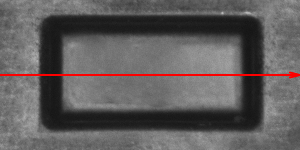
\includegraphics[width=\linewidth]{img/1DEdgeDetection/edges_scan}
    \end{subfigure}%
    ~
    \begin{subfigure}[b]{\basicWidth}
		\smallProfile{img/1DEdgeDetection/edge_profile.values}
    \end{subfigure}
    \caption{1D brightness profile extracted from the image.}
    \label{fig:EdgesProfileExtraction}
\end{figure}

\subsection{Refinement}

\paragraph*{}
Even though a reasonably wide scan area suppresses the noise significantly at the extraction level, we need to keep in mind that only random noise can be suppressed in this way. Real pictures contain small features\footnote{Possibly perpendicular to the scan line and thus not affected by averaging the sampling points.} of image texture irrelevant to the inspection task that need to be attenuated before further processing of the profile. 

\paragraph*{}
Selecting the smoothing filter to refine the extracted profile is not an obvious choice. On the one hand we want to suppress the noise present in the profile, so that irrelevant intensity changes are not identified as edge points, on the other hand we want to achieve high precision of the edge localization. 

\paragraph*{}
These two criteria cannot be considered independently - smoothing of the profile suppresses the noise, but also lowers the precision. Canny determined\cite{Canny86} that the optimal trade-off between noise reduction and lose of precision is achieved with the Gaussian smoothing filter defined as follows:

\[
    g_{\sigma}(x)= \frac{1}{\sqrt{2\pi \sigma^2}} e^{-\frac{x^2}{2 \sigma^2}}
\]

where the standard deviation $\sigma$ is a parameter of the filter.

\subsubsection{Discreet Gaussian Filter}

\paragraph*{}
The Gaussian function is defined in continuous, infinite domain - to obtain a discreet approximation of the filter, we may sample $g_{\sigma}(x)$ at integer coordinates\cite{JainKasturi95}. Moreover, as the value of the Gaussian function quickly decreases with the increase of $|x|$, we may limit the discreet filter to a finite neighborhood of $x = 0$ without significant effect on the results of the smoothing. 

\paragraph*{}
The well known fact called a three-sigma rule states that more that $97\%$ of the Gaussian function integral is concentrated within $3 \sigma$ distance from $x = 0$. It is therefore reasonable to sample the Gaussian function at $2r + 1$ points, where $r$ is a small multiple of $\sigma$, e.g. $3 \lceil \sigma \rceil$; thus obtaining a mask in the following form:

\[
    \frac{1}{s} \begin{bmatrix}
    g(r) & g(r-1) & ... & g(0) & ... & g(r-1) & g(r) 
    \end{bmatrix}
\]

where $s$ equals the sum of the obtained gaussian coefficients, i.e. it ensures the mean-preservation property of the filter.

\subsubsection{Standard Deviation}

\paragraph*{}
Accurate adjustment of $\sigma$ will contribute to the robustness of the computation. We should pick a value that is high enough to eliminate noise that could introduce irrelevant extrema to the profile derivative, but low enough to preserve the actual edges we are to detect. This parameter should be adjusted through interactive experimentation on representative sample data, looking for optimal trade-off between fidelity and noise attenuation. 

\paragraph*{}
\reffig{ProfileSmoothingStdDev} demonstrates effects of smoothing the example brightness profile with different $\sigma$ values. Blue profile ($\sigma = 0.0$) exhibits fine noise while brown profile ($\sigma = 6.0$) attenuates the valleys of significant edges, which makes both suboptimal. Red profile ($\sigma = 3.0$) seems to exhibit appropriate degree of smoothing.

\profileFigure
{
	\addProfileData{img/1DEdgeDetection/edge_profile.values}
	\addProfileData{img/1DEdgeDetection/edge_profile_low_smoothing.values}
	\addProfileData{img/1DEdgeDetection/edge_profile_high_smoothing.values}
}
{Original brightness profile smoothed with different standard deviations of Gaussian operator.}
{ProfileSmoothingStdDev}

